\section{(Alternate) Predicting ELMS in sequences using the API}
\label{sec:predicting_REST}

Querying ELM for motifs in a given sequence (as described in
\ref{sec:predicting_p53} and \ref{sec:predicting_cv_0974}), gives you a nice
overview of putative and possibly
annotated motifs in your query protein with a graphical representation
using colors to highlight different regions of the protein sequence (eg.
disordered vs.~globular). It is however difficult to analyse a large set
of protein sequences in this manner. Therefore, the ELM server
provides an interface which you can use to submit your sequence in a
programmatic way. Of course, this way, you won't receive the graphical
output representation, but are limited to textual data representation.

Currently, there exists a single URL (\code{http://elm.eu.org/start\_search/})
to accept such queries. You can choose to either submit a uniprot name
or accession (eg. \code{http://elm.eu.org/start\_search/P53\_HUMAN.tsv}) or
submit your raw sequence
(e.g.\code{http://elm.eu.org/start\_search/MAPRGFSCLLLLTSEIDLPVKRRA'}.)
If the URL ends in `.tsv' then the server assumes you
are using a Uniprot id or accession; if it doesn't, then it assumes you
are using raw sequence. See below for details.

%
% Subsection: Necessary Resources
%
\subsection{Necessary Resources}
\subsubsection{Software}
A modern browser such as Firefox, Chrome, or Safari. ELM is best viewed
on a laptop or desktop computer, although tablets and smartphones will
also work.
%
There exist several REST client plugins for different browsers, however these
are not needed for this protocol. Ideally use a commandline tool such as
\cl{curl} (\url{http://curl.haxx.se/}) in a terminal window. This program is
available in any of the major operating systems: OSX, Windows and Linux. Of
course, \cl{curl} is only one of many different ways to access web content
programatically, and we suggest to use whichever program you feel is
better suited for your tasks.




\begin{enumerate}

%
% Subsection: Submitting a query via the REST API
%
\subsection{Submitting a query to ELM via the REST API}
\label{subsec:predicting_REST_submitting}

\begin{figure}[h!]
	\centering
	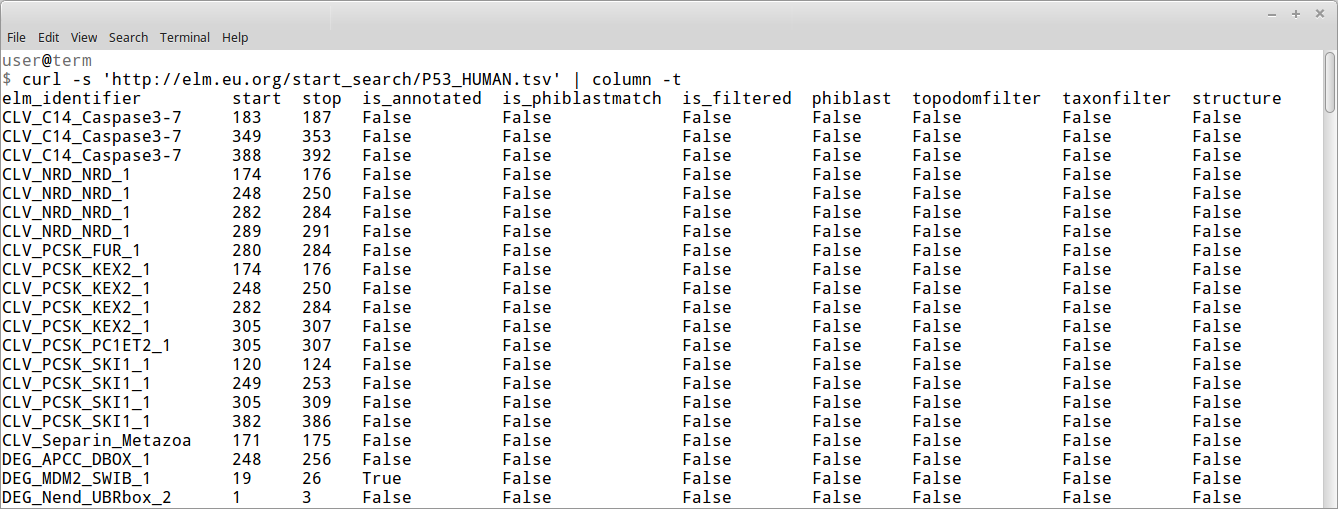
\includegraphics[width=\textwidth]{Figures/predicting_REST/curl_P53.png}
	\caption{
	The commandline output when \code{curl} is used to
	download all motifs predicted in Human P53. Note that we used a more
	advanced command that \code{curl} alone to make the columns align
	nicely (see text for an explanation).
	}
	\label{fig:predicting_REST_curl_p53}
\end{figure}


\item Use \code{curl} to query ELM for all motifs predicted to occur in Human
	P53 by typing the following into a terminal: `curl
	`http://elm.eu.org/start\_search/P53\_HUMAN.tsv'. Each row represents a
	motif detection, and the first column ``elm\_identifier'' indicates
	which class was identified. The columns ``start'' and ``stop'' show
	that first and last amino acid positions that matched form part of the
	motif.  Column ``is annotated'' is True if this motif has been
	annotated in the database as an (experimentally validated) motif
	instance. The coulmn ``is phiblastmatch'' is True if ?????. The column
	``is filtered'' shows whether or not this motif was rejected by the
	ELM Prediction structure filter. Coulumn ``phibast'' indicates whether
	?????.  The ``topodomfilter'' and ``taxonfilter'' shown whether ?????.
	The last column ``structure'' ?????

	\sdesc{In figure \ref{fig:predicting_REST_curl_p53}
		we use a slightly more
		advanced command to get the output to look nice in the
		terminal. We specified the \code{-s} option to silence all
		\code{curl} output other than the downloaded file, and piped
		the output directly to the
		\code{column} command (this command exists on most Linux and
		OSX machines).}

TODO: Holger: what are the columns that are not described in the above section for?

\begin{figure}[h!]
	\centering
	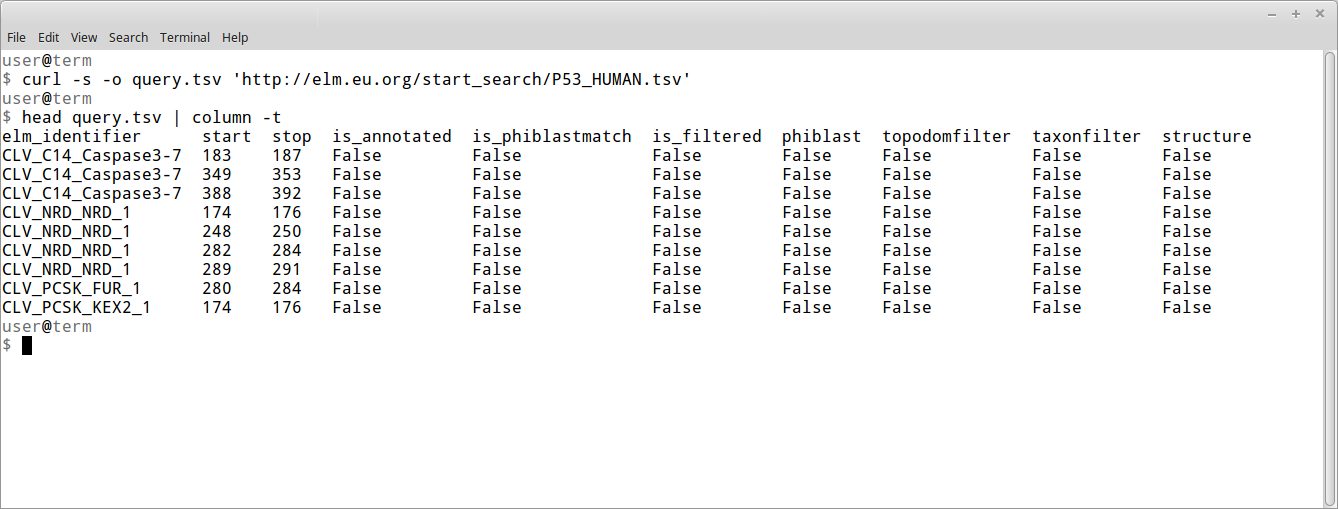
\includegraphics[width=\textwidth]{Figures/predicting_REST/predictions_query.png} 
	\caption{
	It is possible to send amino acid sequences to the ELM Prediction
	pipeline. In this case we have used
	the curl option \code{-o} to download directly to the file
	\code{query.tsv}, and use a combination of the \code{head} and
	\code{column} commands to display the first 10 rows to the terminal.
	}
	\label{fig:predicting_REST_query}
\end{figure}

\item Use \code{curl} to query ELM via protein sequence by using the URL
	\code{http://elm.eu.org/start\_search/MAPRGFSCLLLLTSEIDLPVKRRA}
	(Fig. \ref{fig:predicting_REST_query}).
	In this case the query is an arbitrary short
	peptide sequence, but this can (of course) contain any sequence you are
	interested in analysing. The output format is exactly the same as in the
	previous step.

	\sdesc{ This way of querying ELM is unfortunately not stable for long
		protein sequences. Different browsers and computers have
		different maximum lengths for URLs, and the excess text is
		often simply ignored. We recommend not using this method for
		sequences longer than 2000 amino acids.}

\end{enumerate}
